%==============================================================================
%  Tu propio servicio de LLM — seminario, Máster en Desarrollo del Software (UGR)
%  Estilo: latexUGR v2 (divulgación).  Compilar dos veces con pdflatex.
%  Por defecto genera presentacion.pdf sin notas; para presentacion-notas.pdf:
%  pdflatex -jobname=presentacion-notas '\def\showpresenternotes{1}%==============================================================================
%  Tu propio servicio de LLM — seminario, Máster en Desarrollo del Software (UGR)
%  Estilo: latexUGR v2 (divulgación).  Compilar dos veces con pdflatex.
%  Por defecto genera presentacion.pdf sin notas; para presentacion-notas.pdf:
%  pdflatex -jobname=presentacion-notas '\def\showpresenternotes{1}%==============================================================================
%  Tu propio servicio de LLM — seminario, Máster en Desarrollo del Software (UGR)
%  Estilo: latexUGR v2 (divulgación).  Compilar dos veces con pdflatex.
%  Por defecto genera presentacion.pdf sin notas; para presentacion-notas.pdf:
%  pdflatex -jobname=presentacion-notas '\def\showpresenternotes{1}%==============================================================================
%  Tu propio servicio de LLM — seminario, Máster en Desarrollo del Software (UGR)
%  Estilo: latexUGR v2 (divulgación).  Compilar dos veces con pdflatex.
%  Por defecto genera presentacion.pdf sin notas; para presentacion-notas.pdf:
%  pdflatex -jobname=presentacion-notas '\def\showpresenternotes{1}\input{presentacion.tex}'
%  Los bloques están en p1_why.tex ... p7_wrapup.tex (se incluyen más abajo).
%  Las ilustraciones van en imagenes/ (ver imagenes/PROMPTS.md); si un fichero
%  no existe, el documento compila igual y muestra un marcador con su nombre.
%
%  Nota: si el entorno no tiene babel-spanish, se usa babel [english] con
%  UTF-8 y sin partición de palabras (la elección es automática).
%==============================================================================
\documentclass[aspectratio=169,11pt]{beamer}
\ifdefined\showpresenternotes
  \setbeameroption{show notes on second screen=right}
\else
  \setbeameroption{hide notes}
\fi

\usepackage[utf8]{inputenc}
\usepackage[T1]{fontenc}
\usepackage{lmodern}
\IfFileExists{spanish.ldf}{%
  \usepackage[spanish,es-noshorthands]{babel}}{%
  \usepackage[english]{babel}\hyphenpenalty=10000 \exhyphenpenalty=10000}
\usepackage{latexUGR}
\usepackage{amssymb}
\usepackage{listings}
\usepackage{array}

\ugrfooter{LLM on-premise · Universidad de Granada}
\ugrlogo{imagenes/logoUGR.png}
\IfFileExists{imagenes/portada.png}{\ugrcover{imagenes/portada.png}}{%
  \IfFileExists{imagenes/portada.jpg}{\ugrcover{imagenes/portada.jpg}}{}}

\title[LLM on-premise]{Infraestructura LLM on-premise}
\subtitle{Inferencia, gateways, agentes y MCP}
\author[I. Vidal Daza]{Isaac Vidal Daza}
\institute[UGR]{Servicio de Apoyo a la Docencia, CSIRC \\ Universidad de Granada}
\date{Máster en Desarrollo del Software · Granada, 2026}

%------------------------------------------------------------------ estilos compartidos
\newcolumntype{R}[1]{>{\raggedright\arraybackslash}p{#1}}

% Diagramas TikZ: cajas planas con borde fino, en la paleta de la plantilla v2
\tikzset{
  bx/.style={rounded corners=4pt, draw=ugrLine, fill=ugrSand, line width=0.8pt,
             align=center, font=\footnotesize, text=ugrInk, inner sep=4pt, minimum height=0.8cm},
  rbx/.style={bx, draw=rojoUGR, fill=rojoUGR!8},
  bbx/.style={bx, draw=nA, fill=nA!8},
  gbx/.style={bx, draw=nB, fill=nB!8},
  pbx/.style={bx, draw=nD, fill=nD!8},
  abx/.style={bx, draw=nE, fill=nE!8},
  ar/.style={-{Stealth[length=4pt]}, line width=0.9pt, draw=ugrText},
  bar/.style={{Stealth[length=4pt]}-{Stealth[length=4pt]}, line width=0.9pt, draw=ugrText},
  lab/.style={font=\footnotesize\itshape, text=darkgray},
}

% Código: fondo arena y barra roja a la izquierda (como la barra del título)
\lstdefinestyle{ugr}{
  basicstyle=\ttfamily\fontsize{6.9}{8.2}\selectfont\color{ugrInk},
  keywordstyle=\color{rojoDark},
  commentstyle=\color{nGreen}\itshape,
  stringstyle=\color{nA},
  backgroundcolor=\color{ugrSand},
  frame=l, framerule=2.5pt, rulecolor=\color{rojoUGR}, framesep=6pt,
  showstringspaces=false, columns=fullflexible, keepspaces=true,
  xleftmargin=10pt, xrightmargin=0pt, aboveskip=2pt, belowskip=2pt,
  breaklines=true, language=Python,
  extendedchars=true, inputencoding=utf8,
  literate={á}{{\'a}}1 {é}{{\'e}}1 {í}{{\'i}}1 {ó}{{\'o}}1 {ú}{{\'u}}1
           {ñ}{{\~n}}1 {Á}{{\'A}}1 {É}{{\'E}}1 {Í}{{\'I}}1 {Ó}{{\'O}}1 {Ú}{{\'U}}1
           {Ñ}{{\~N}}1 {¿}{{?`}}1 {¡}{{!`}}1 {«}{{\guillemotleft}}1 {»}{{\guillemotright}}1
           {·}{{\textperiodcentered}}1 {…}{{\ldots}}1 {→}{{$\rightarrow$}}1
           {ª}{{\textordfeminine}}1,
}
\lstset{style=ugr}

% Chip verde de demo:  \demochip{nombre del script}
\newcommand{\demochip}[1]{%
  \begin{tikzpicture}
    \node[rounded corners=7pt, fill=nB, text=white, font=\scriptsize\bfseries,
          inner xsep=7pt, inner ysep=3pt]
      {$\blacktriangleright$\ Demo: \texttt{#1}};
  \end{tikzpicture}}
\newcommand{\demoline}[1]{\par\vspace{2pt}\hfill\demochip{#1}\par}

% Línea de fuentes al pie de un frame
\newcommand{\srcline}[1]{{\par\vspace{2pt}\tiny\color{darkgray}Fuentes: #1\par}}

% Ilustración con marcador: usa imagenes/<fichero> si existe; si no, muestra un
% recuadro con el nombre y la descripción (así el documento siempre compila).
%   \imgslot{fichero}{ancho}{alto}{descripción del marcador}
\newcommand{\imgslot}[4]{%
  \IfFileExists{imagenes/#1}{%
    \includegraphics[width=#2,height=#3,keepaspectratio]{imagenes/#1}}{%
    \begin{tikzpicture}
      \node[draw=darkgray!50, dashed, line width=0.8pt, fill=ugrSand, rounded corners=5pt,
            minimum width=#2, minimum height=#3, text width=\dimexpr#2-0.8cm\relax,
            align=center, text=darkgray, font=\scriptsize]
        {\textbf{Imagen pendiente}\\[1pt] \texttt{\detokenize{imagenes/#1}}\\[3pt] #4};
    \end{tikzpicture}}}

\begin{document}

%--------------------------------------------------------------- portada
\newcommand{\portadarepo}{%
  \tikz[remember picture,overlay] \node[anchor=south west,inner sep=0pt,align=left]
    at ([xshift=4.2cm,yshift=0.7cm]current page.south west)
    {\footnotesize Presentación, código y ejemplos:\\
     \footnotesize\color{nA}\href{https://github.com/isvida/MiIA-demo}{\texttt{https://github.com/isvida/MiIA-demo}}};}
\ugrtitleframe[\ugrtag{Inferencia}\hspace{4pt}\ugrtag{Pasarela}\hspace{4pt}\ugrtag{Agentes}\hspace{4pt}\ugrtag{MCP}\smash{\portadarepo}]

%--------------------------------------------------------------- frase de apertura
\ugrstatement{Un modelo de lenguaje ya no es un experimento: es una pieza más de la infraestructura, como el correo o las bases de datos.}{Punto de partida de este seminario}

%--------------------------------------------------------------- agenda
\begin{frame}{Agenda}{Tiempo transcurrido previsto al comenzar cada bloque · formato h:mm}
	\note{Dos horas; señalar el orden y las demos.}
	\vspace{0.1cm}
	\begin{tikzpicture}
		\foreach \n/\t/\m/\p [count=\i] in {
		1/{¿Por qué tener tu propio LLM?}/{0:00}/{},
		2/{Motores de inferencia}/{0:10}/{01\_hola\_api · 02\_concurrencia},
		3/{Hablar con un LLM}/{0:30}/{03\_salida · 04\_tool\_calling},
		4/{Arquitectura del servicio}/{0:45}/{pasarela, claves, respaldo},
		5/{Agentes, MCP y skills}/{1:05}/{05\_agente · 06\_agente\_mcp},
		6/{Casos de uso}/{1:30}/{03 (patrón EPFReader)},
		7/{Conclusiones y preguntas}/{1:50}/{}}{
		\pgfmathsetmacro{\yy}{-(\i-1)*0.62}
		\node[fill=rojoUGR, text=white, font=\scriptsize\bfseries, minimum size=0.48cm,
			rounded corners=1.5pt, anchor=west] at (0,\yy) {\n};
		\node[anchor=west, text=ugrInk, font=\normalsize\bfseries] at (0.75,\yy) {\t};
		\node[anchor=east, text=rojoUGR, font=\small\bfseries] at (8.3,\yy) {\m};
		\node[anchor=west, text=darkgray, font=\scriptsize] at (8.8,\yy) {\p};
		}
		\draw[ugrLine, line width=1pt] (0,-4.15) -- (13.8,-4.15);
		\node[anchor=west, text=ugrInk, font=\normalsize\bfseries] at (0.75,-4.5) {Fin previsto};
		\node[anchor=east, text=rojoUGR, font=\small\bfseries] at (8.3,-4.5) {2:00};
	\end{tikzpicture}
\end{frame}

%--------------------------------------------------------------- puesta en marcha
\begin{frame}[fragile]{Antes de empezar: levanta la demo}{Una miniatura de la infraestructura real, sin necesidad de GPU}
	\note{Dejar la descarga en marcha; servicios locales y URL de acceso.}
	\begin{columns}[T]
		\begin{column}{0.56\textwidth}
			\begin{lstlisting}[language={}]
unzip miia-demo.zip && cd miia-demo
docker compose pull
docker compose build
docker compose up -d
docker compose run --rm lab \
    python ejemplos/01_hola_api.py
\end{lstlisting}
			\vspace{6pt}
			{\footnotesize Requiere Docker con Compose v2, unos 8 GB de RAM libres y unos 6 GB de disco.
				Hay un perfil opcional con GPU y vLLM.}
		\end{column}
		\begin{column}{0.42\textwidth}
			\themeblock{nA}{Qué se levanta, y dónde}{%
				Chat (Open WebUI): \texttt{localhost:3000}\\
				Panel de LiteLLM: \texttt{localhost:4000/ui}\\
				API tipo OpenAI: \texttt{localhost:4000/v1}\\
				Servidor MCP: \texttt{localhost:8001/mcp}}
		\end{column}
	\end{columns}
	\keymsg{Lanza la descarga ya: se completa mientras vemos el bloque 1.}
\end{frame}

%--------------------------------------------------------------- bloques
\InputIfFileExists{p1_why.tex}{}{}
\InputIfFileExists{p2_inference.tex}{}{}
\InputIfFileExists{p3_api.tex}{}{}
\InputIfFileExists{p4_architecture.tex}{}{}
\InputIfFileExists{p5_agents.tex}{}{}
\InputIfFileExists{p6_usecases.tex}{}{}
\InputIfFileExists{p7_wrapup.tex}{}{}

%--------------------------------------------------------------- invitación al MOOC
\ugrimageframe{imagenes/equipo_gobierno_mia.png}
  {¿Podría MiIA tomar el control de la UGR y sustituir al equipo de gobierno?}
  {Una pregunta para mirar más allá de la automatización.}

\ugrimageframe{imagenes/mooc.png}
  {¿Quieres la respuesta? Apúntate al MOOC del CEPRUD}
  {\footnotesize Capítulo: Inteligencia artificial y evolución: modelando un sistema vivo artificial\\
   Coorganizan: Isaac Vidal Daza y Mónica Sánchez-Román (Mineralogía y Petrología, UGR)\\
   Posible apertura de matrícula en diciembre.}

\begin{frame}{Agradecimientos}{CSIRC · Apoyo a la Docencia}
  \note{Equipo de apoyo a la docencia del CSIRC.}
  \centering
  \begin{tikzpicture}[
    persona/.style={bx, text width=3.4cm, minimum height=0.7cm,
                    font=\footnotesize, inner sep=3pt},
    centro/.style={rbx, text width=3.0cm, minimum height=1.0cm,
                   font=\small\bfseries, inner sep=4pt},
    enlace/.style={draw=ugrLine, line width=0.9pt}
  ]
    \node[centro] (francisco) at (0,0) {Francisco Manuel\\Romera Juárez};
    \node[persona] (domingo) at (-4.2,1.5) {Domingo de Guzmán\\Baca Ruiz};
    \node[persona] (antonio) at (-4.2,0.5) {Antonio Ángel\\Cano Ruano};
    \node[persona] (rodrigo) at (-4.2,-0.5) {Rodrigo González\\Gálvez};
    \node[persona] (fernando) at (-4.2,-1.5) {Fernando Antonio\\López Álvarez};
    \node[persona] (leire) at (4.2,1.5) {Leire Melchor López};
    \node[persona] (gines) at (4.2,0.5) {Ginés Rubio Flores};
    \node[persona] (ruiz) at (4.2,-0.5) {Antonio Ruiz González};
    \node[persona] (isaac) at (4.2,-1.5) {Isaac Vidal Daza};
    \begin{scope}[on background layer]
      \foreach \persona in {domingo,antonio,rodrigo,fernando,leire,gines,ruiz,isaac}
        \draw[enlace] (francisco) -- (\persona);
    \end{scope}
  \end{tikzpicture}

  \vspace{3pt}
  {\scriptsize Centro de Servicios Informáticos y Redes de Comunicación\\
  Servicio Central de Informática (Edf. Mecenas) · C/ Profesor Adolfo Rancaño,
  18071 Granada\\
  \href{http://csirc.ugr.es}{\textcolor{nA}{csirc.ugr.es}}}
\end{frame}

\begin{frame}{Agradecimientos}{Cátedra GPU Solutions-UGR}
  \note{Agradecer el apoyo y el equipamiento de la Cátedra.}
  \begin{columns}[c]
    \begin{column}{0.53\textwidth}
      \centering
      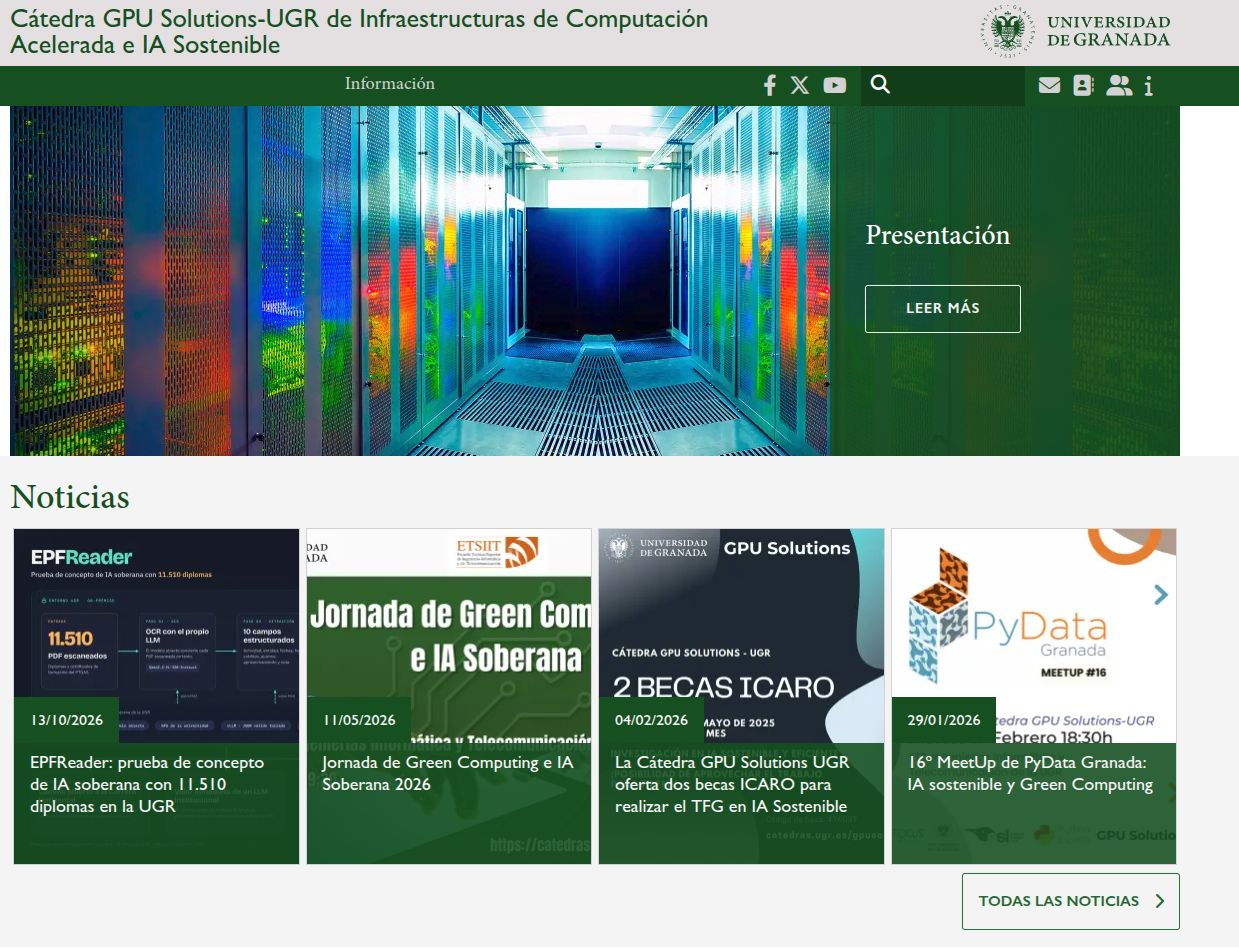
\includegraphics[width=\linewidth,height=5cm,keepaspectratio]{imagenes/catedra.png}\\[6pt]
      {\scriptsize\href{https://catedras.ugr.es/gpusolutions/}{\textcolor{nA}{\texttt{https://catedras.ugr.es/gpusolutions/}}}}
    \end{column}
    \begin{column}{0.45\textwidth}
      \themeblock{rojoUGR}{Gracias}{%
        A la\\\textbf{\mbox{Cátedra GPU Solutions-UGR}}\\
        por el apoyo y el equipamiento facilitado para el desarrollo de MiIA.}
    \end{column}
  \end{columns}
\end{frame}

%=============================================================== cierre
\ugrthanks{¡Gracias!}{¿Preguntas?}{%
  \textbf{Isaac Vidal Daza}\\
  Servicio de Apoyo a la Docencia · CSIRC\\
  \textcolor{rojoUGR}{isvida@ugr.es}\\[12pt]
  {\Large\bfseries\color{ugrInk}   \href{https://www.ugr.es/~isvida}{\texttt{https://www.ugr.es/\raisebox{0.5ex}{\texttildelow}isvida}}}}{}


\end{document}
'
%  Los bloques están en p1_why.tex ... p7_wrapup.tex (se incluyen más abajo).
%  Las ilustraciones van en imagenes/ (ver imagenes/PROMPTS.md); si un fichero
%  no existe, el documento compila igual y muestra un marcador con su nombre.
%
%  Nota: si el entorno no tiene babel-spanish, se usa babel [english] con
%  UTF-8 y sin partición de palabras (la elección es automática).
%==============================================================================
\documentclass[aspectratio=169,11pt]{beamer}
\ifdefined\showpresenternotes
  \setbeameroption{show notes on second screen=right}
\else
  \setbeameroption{hide notes}
\fi

\usepackage[utf8]{inputenc}
\usepackage[T1]{fontenc}
\usepackage{lmodern}
\IfFileExists{spanish.ldf}{%
  \usepackage[spanish,es-noshorthands]{babel}}{%
  \usepackage[english]{babel}\hyphenpenalty=10000 \exhyphenpenalty=10000}
\usepackage{latexUGR}
\usepackage{amssymb}
\usepackage{listings}
\usepackage{array}

\ugrfooter{LLM on-premise · Universidad de Granada}
\ugrlogo{imagenes/logoUGR.png}
\IfFileExists{imagenes/portada.png}{\ugrcover{imagenes/portada.png}}{%
  \IfFileExists{imagenes/portada.jpg}{\ugrcover{imagenes/portada.jpg}}{}}

\title[LLM on-premise]{Infraestructura LLM on-premise}
\subtitle{Inferencia, gateways, agentes y MCP}
\author[I. Vidal Daza]{Isaac Vidal Daza}
\institute[UGR]{Servicio de Apoyo a la Docencia, CSIRC \\ Universidad de Granada}
\date{Máster en Desarrollo del Software · Granada, 2026}

%------------------------------------------------------------------ estilos compartidos
\newcolumntype{R}[1]{>{\raggedright\arraybackslash}p{#1}}

% Diagramas TikZ: cajas planas con borde fino, en la paleta de la plantilla v2
\tikzset{
  bx/.style={rounded corners=4pt, draw=ugrLine, fill=ugrSand, line width=0.8pt,
             align=center, font=\footnotesize, text=ugrInk, inner sep=4pt, minimum height=0.8cm},
  rbx/.style={bx, draw=rojoUGR, fill=rojoUGR!8},
  bbx/.style={bx, draw=nA, fill=nA!8},
  gbx/.style={bx, draw=nB, fill=nB!8},
  pbx/.style={bx, draw=nD, fill=nD!8},
  abx/.style={bx, draw=nE, fill=nE!8},
  ar/.style={-{Stealth[length=4pt]}, line width=0.9pt, draw=ugrText},
  bar/.style={{Stealth[length=4pt]}-{Stealth[length=4pt]}, line width=0.9pt, draw=ugrText},
  lab/.style={font=\footnotesize\itshape, text=darkgray},
}

% Código: fondo arena y barra roja a la izquierda (como la barra del título)
\lstdefinestyle{ugr}{
  basicstyle=\ttfamily\fontsize{6.9}{8.2}\selectfont\color{ugrInk},
  keywordstyle=\color{rojoDark},
  commentstyle=\color{nGreen}\itshape,
  stringstyle=\color{nA},
  backgroundcolor=\color{ugrSand},
  frame=l, framerule=2.5pt, rulecolor=\color{rojoUGR}, framesep=6pt,
  showstringspaces=false, columns=fullflexible, keepspaces=true,
  xleftmargin=10pt, xrightmargin=0pt, aboveskip=2pt, belowskip=2pt,
  breaklines=true, language=Python,
  extendedchars=true, inputencoding=utf8,
  literate={á}{{\'a}}1 {é}{{\'e}}1 {í}{{\'i}}1 {ó}{{\'o}}1 {ú}{{\'u}}1
           {ñ}{{\~n}}1 {Á}{{\'A}}1 {É}{{\'E}}1 {Í}{{\'I}}1 {Ó}{{\'O}}1 {Ú}{{\'U}}1
           {Ñ}{{\~N}}1 {¿}{{?`}}1 {¡}{{!`}}1 {«}{{\guillemotleft}}1 {»}{{\guillemotright}}1
           {·}{{\textperiodcentered}}1 {…}{{\ldots}}1 {→}{{$\rightarrow$}}1
           {ª}{{\textordfeminine}}1,
}
\lstset{style=ugr}

% Chip verde de demo:  \demochip{nombre del script}
\newcommand{\demochip}[1]{%
  \begin{tikzpicture}
    \node[rounded corners=7pt, fill=nB, text=white, font=\scriptsize\bfseries,
          inner xsep=7pt, inner ysep=3pt]
      {$\blacktriangleright$\ Demo: \texttt{#1}};
  \end{tikzpicture}}
\newcommand{\demoline}[1]{\par\vspace{2pt}\hfill\demochip{#1}\par}

% Línea de fuentes al pie de un frame
\newcommand{\srcline}[1]{{\par\vspace{2pt}\tiny\color{darkgray}Fuentes: #1\par}}

% Ilustración con marcador: usa imagenes/<fichero> si existe; si no, muestra un
% recuadro con el nombre y la descripción (así el documento siempre compila).
%   \imgslot{fichero}{ancho}{alto}{descripción del marcador}
\newcommand{\imgslot}[4]{%
  \IfFileExists{imagenes/#1}{%
    \includegraphics[width=#2,height=#3,keepaspectratio]{imagenes/#1}}{%
    \begin{tikzpicture}
      \node[draw=darkgray!50, dashed, line width=0.8pt, fill=ugrSand, rounded corners=5pt,
            minimum width=#2, minimum height=#3, text width=\dimexpr#2-0.8cm\relax,
            align=center, text=darkgray, font=\scriptsize]
        {\textbf{Imagen pendiente}\\[1pt] \texttt{\detokenize{imagenes/#1}}\\[3pt] #4};
    \end{tikzpicture}}}

\begin{document}

%--------------------------------------------------------------- portada
\newcommand{\portadarepo}{%
  \tikz[remember picture,overlay] \node[anchor=south west,inner sep=0pt,align=left]
    at ([xshift=4.2cm,yshift=0.7cm]current page.south west)
    {\footnotesize Presentación, código y ejemplos:\\
     \footnotesize\color{nA}\href{https://github.com/isvida/MiIA-demo}{\texttt{https://github.com/isvida/MiIA-demo}}};}
\ugrtitleframe[\ugrtag{Inferencia}\hspace{4pt}\ugrtag{Pasarela}\hspace{4pt}\ugrtag{Agentes}\hspace{4pt}\ugrtag{MCP}\smash{\portadarepo}]

%--------------------------------------------------------------- frase de apertura
\ugrstatement{Un modelo de lenguaje ya no es un experimento: es una pieza más de la infraestructura, como el correo o las bases de datos.}{Punto de partida de este seminario}

%--------------------------------------------------------------- agenda
\begin{frame}{Agenda}{Tiempo transcurrido previsto al comenzar cada bloque · formato h:mm}
	\note{Dos horas; señalar el orden y las demos.}
	\vspace{0.1cm}
	\begin{tikzpicture}
		\foreach \n/\t/\m/\p [count=\i] in {
		1/{¿Por qué tener tu propio LLM?}/{0:00}/{},
		2/{Motores de inferencia}/{0:10}/{01\_hola\_api · 02\_concurrencia},
		3/{Hablar con un LLM}/{0:30}/{03\_salida · 04\_tool\_calling},
		4/{Arquitectura del servicio}/{0:45}/{pasarela, claves, respaldo},
		5/{Agentes, MCP y skills}/{1:05}/{05\_agente · 06\_agente\_mcp},
		6/{Casos de uso}/{1:30}/{03 (patrón EPFReader)},
		7/{Conclusiones y preguntas}/{1:50}/{}}{
		\pgfmathsetmacro{\yy}{-(\i-1)*0.62}
		\node[fill=rojoUGR, text=white, font=\scriptsize\bfseries, minimum size=0.48cm,
			rounded corners=1.5pt, anchor=west] at (0,\yy) {\n};
		\node[anchor=west, text=ugrInk, font=\normalsize\bfseries] at (0.75,\yy) {\t};
		\node[anchor=east, text=rojoUGR, font=\small\bfseries] at (8.3,\yy) {\m};
		\node[anchor=west, text=darkgray, font=\scriptsize] at (8.8,\yy) {\p};
		}
		\draw[ugrLine, line width=1pt] (0,-4.15) -- (13.8,-4.15);
		\node[anchor=west, text=ugrInk, font=\normalsize\bfseries] at (0.75,-4.5) {Fin previsto};
		\node[anchor=east, text=rojoUGR, font=\small\bfseries] at (8.3,-4.5) {2:00};
	\end{tikzpicture}
\end{frame}

%--------------------------------------------------------------- puesta en marcha
\begin{frame}[fragile]{Antes de empezar: levanta la demo}{Una miniatura de la infraestructura real, sin necesidad de GPU}
	\note{Dejar la descarga en marcha; servicios locales y URL de acceso.}
	\begin{columns}[T]
		\begin{column}{0.56\textwidth}
			\begin{lstlisting}[language={}]
unzip miia-demo.zip && cd miia-demo
docker compose pull
docker compose build
docker compose up -d
docker compose run --rm lab \
    python ejemplos/01_hola_api.py
\end{lstlisting}
			\vspace{6pt}
			{\footnotesize Requiere Docker con Compose v2, unos 8 GB de RAM libres y unos 6 GB de disco.
				Hay un perfil opcional con GPU y vLLM.}
		\end{column}
		\begin{column}{0.42\textwidth}
			\themeblock{nA}{Qué se levanta, y dónde}{%
				Chat (Open WebUI): \texttt{localhost:3000}\\
				Panel de LiteLLM: \texttt{localhost:4000/ui}\\
				API tipo OpenAI: \texttt{localhost:4000/v1}\\
				Servidor MCP: \texttt{localhost:8001/mcp}}
		\end{column}
	\end{columns}
	\keymsg{Lanza la descarga ya: se completa mientras vemos el bloque 1.}
\end{frame}

%--------------------------------------------------------------- bloques
\InputIfFileExists{p1_why.tex}{}{}
\InputIfFileExists{p2_inference.tex}{}{}
\InputIfFileExists{p3_api.tex}{}{}
\InputIfFileExists{p4_architecture.tex}{}{}
\InputIfFileExists{p5_agents.tex}{}{}
\InputIfFileExists{p6_usecases.tex}{}{}
\InputIfFileExists{p7_wrapup.tex}{}{}

%--------------------------------------------------------------- invitación al MOOC
\ugrimageframe{imagenes/equipo_gobierno_mia.png}
  {¿Podría MiIA tomar el control de la UGR y sustituir al equipo de gobierno?}
  {Una pregunta para mirar más allá de la automatización.}

\ugrimageframe{imagenes/mooc.png}
  {¿Quieres la respuesta? Apúntate al MOOC del CEPRUD}
  {\footnotesize Capítulo: Inteligencia artificial y evolución: modelando un sistema vivo artificial\\
   Coorganizan: Isaac Vidal Daza y Mónica Sánchez-Román (Mineralogía y Petrología, UGR)\\
   Posible apertura de matrícula en diciembre.}

\begin{frame}{Agradecimientos}{CSIRC · Apoyo a la Docencia}
  \note{Equipo de apoyo a la docencia del CSIRC.}
  \centering
  \begin{tikzpicture}[
    persona/.style={bx, text width=3.4cm, minimum height=0.7cm,
                    font=\footnotesize, inner sep=3pt},
    centro/.style={rbx, text width=3.0cm, minimum height=1.0cm,
                   font=\small\bfseries, inner sep=4pt},
    enlace/.style={draw=ugrLine, line width=0.9pt}
  ]
    \node[centro] (francisco) at (0,0) {Francisco Manuel\\Romera Juárez};
    \node[persona] (domingo) at (-4.2,1.5) {Domingo de Guzmán\\Baca Ruiz};
    \node[persona] (antonio) at (-4.2,0.5) {Antonio Ángel\\Cano Ruano};
    \node[persona] (rodrigo) at (-4.2,-0.5) {Rodrigo González\\Gálvez};
    \node[persona] (fernando) at (-4.2,-1.5) {Fernando Antonio\\López Álvarez};
    \node[persona] (leire) at (4.2,1.5) {Leire Melchor López};
    \node[persona] (gines) at (4.2,0.5) {Ginés Rubio Flores};
    \node[persona] (ruiz) at (4.2,-0.5) {Antonio Ruiz González};
    \node[persona] (isaac) at (4.2,-1.5) {Isaac Vidal Daza};
    \begin{scope}[on background layer]
      \foreach \persona in {domingo,antonio,rodrigo,fernando,leire,gines,ruiz,isaac}
        \draw[enlace] (francisco) -- (\persona);
    \end{scope}
  \end{tikzpicture}

  \vspace{3pt}
  {\scriptsize Centro de Servicios Informáticos y Redes de Comunicación\\
  Servicio Central de Informática (Edf. Mecenas) · C/ Profesor Adolfo Rancaño,
  18071 Granada\\
  \href{http://csirc.ugr.es}{\textcolor{nA}{csirc.ugr.es}}}
\end{frame}

\begin{frame}{Agradecimientos}{Cátedra GPU Solutions-UGR}
  \note{Agradecer el apoyo y el equipamiento de la Cátedra.}
  \begin{columns}[c]
    \begin{column}{0.53\textwidth}
      \centering
      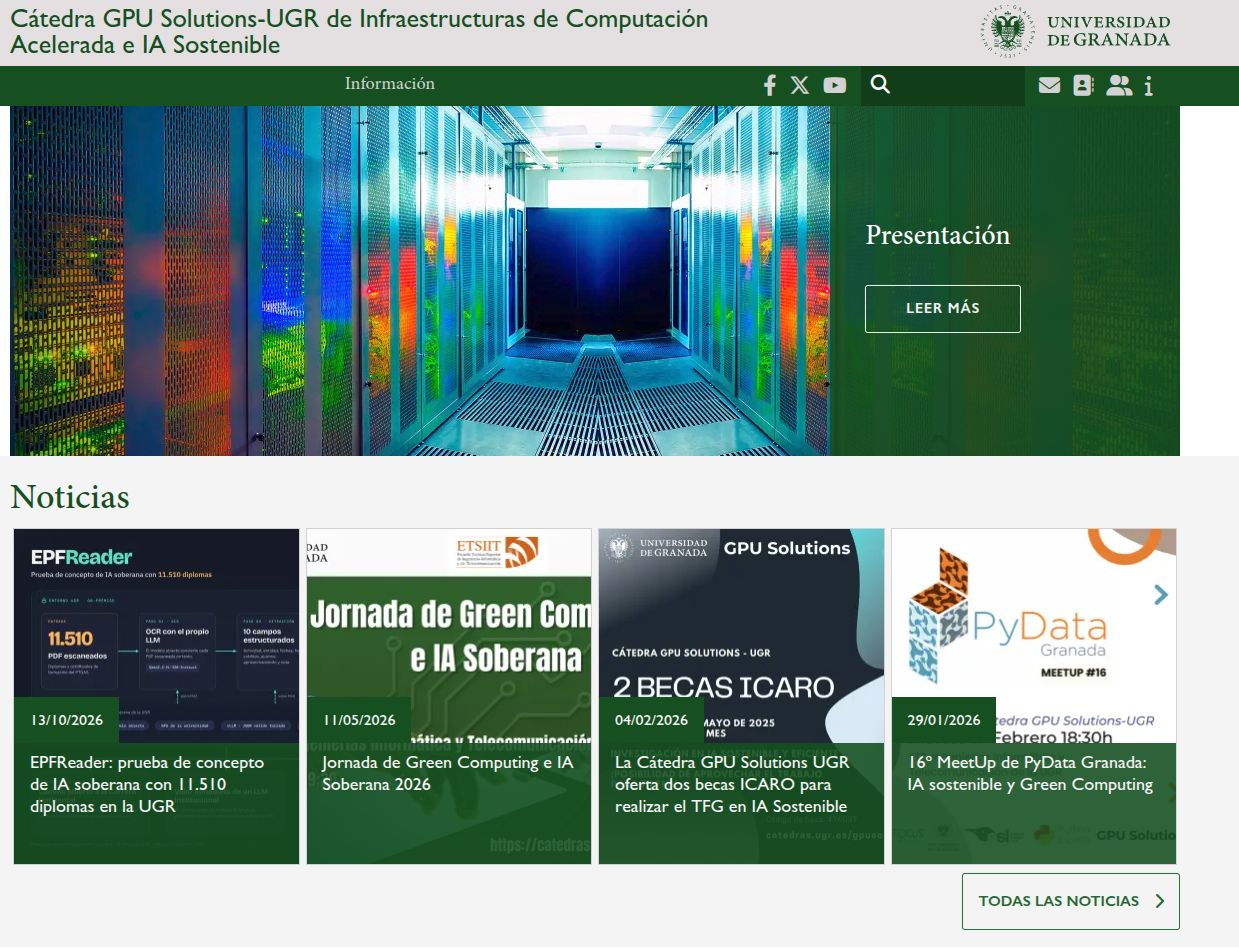
\includegraphics[width=\linewidth,height=5cm,keepaspectratio]{imagenes/catedra.png}\\[6pt]
      {\scriptsize\href{https://catedras.ugr.es/gpusolutions/}{\textcolor{nA}{\texttt{https://catedras.ugr.es/gpusolutions/}}}}
    \end{column}
    \begin{column}{0.45\textwidth}
      \themeblock{rojoUGR}{Gracias}{%
        A la\\\textbf{\mbox{Cátedra GPU Solutions-UGR}}\\
        por el apoyo y el equipamiento facilitado para el desarrollo de MiIA.}
    \end{column}
  \end{columns}
\end{frame}

%=============================================================== cierre
\ugrthanks{¡Gracias!}{¿Preguntas?}{%
  \textbf{Isaac Vidal Daza}\\
  Servicio de Apoyo a la Docencia · CSIRC\\
  \textcolor{rojoUGR}{isvida@ugr.es}\\[12pt]
  {\Large\bfseries\color{ugrInk}   \href{https://www.ugr.es/~isvida}{\texttt{https://www.ugr.es/\raisebox{0.5ex}{\texttildelow}isvida}}}}{}


\end{document}
'
%  Los bloques están en p1_why.tex ... p7_wrapup.tex (se incluyen más abajo).
%  Las ilustraciones van en imagenes/ (ver imagenes/PROMPTS.md); si un fichero
%  no existe, el documento compila igual y muestra un marcador con su nombre.
%
%  Nota: si el entorno no tiene babel-spanish, se usa babel [english] con
%  UTF-8 y sin partición de palabras (la elección es automática).
%==============================================================================
\documentclass[aspectratio=169,11pt]{beamer}
\ifdefined\showpresenternotes
  \setbeameroption{show notes on second screen=right}
\else
  \setbeameroption{hide notes}
\fi

\usepackage[utf8]{inputenc}
\usepackage[T1]{fontenc}
\usepackage{lmodern}
\IfFileExists{spanish.ldf}{%
  \usepackage[spanish,es-noshorthands]{babel}}{%
  \usepackage[english]{babel}\hyphenpenalty=10000 \exhyphenpenalty=10000}
\usepackage{latexUGR}
\usepackage{amssymb}
\usepackage{listings}
\usepackage{array}

\ugrfooter{LLM on-premise · Universidad de Granada}
\ugrlogo{imagenes/logoUGR.png}
\IfFileExists{imagenes/portada.png}{\ugrcover{imagenes/portada.png}}{%
  \IfFileExists{imagenes/portada.jpg}{\ugrcover{imagenes/portada.jpg}}{}}

\title[LLM on-premise]{Infraestructura LLM on-premise}
\subtitle{Inferencia, gateways, agentes y MCP}
\author[I. Vidal Daza]{Isaac Vidal Daza}
\institute[UGR]{Servicio de Apoyo a la Docencia, CSIRC \\ Universidad de Granada}
\date{Máster en Desarrollo del Software · Granada, 2026}

%------------------------------------------------------------------ estilos compartidos
\newcolumntype{R}[1]{>{\raggedright\arraybackslash}p{#1}}

% Diagramas TikZ: cajas planas con borde fino, en la paleta de la plantilla v2
\tikzset{
  bx/.style={rounded corners=4pt, draw=ugrLine, fill=ugrSand, line width=0.8pt,
             align=center, font=\footnotesize, text=ugrInk, inner sep=4pt, minimum height=0.8cm},
  rbx/.style={bx, draw=rojoUGR, fill=rojoUGR!8},
  bbx/.style={bx, draw=nA, fill=nA!8},
  gbx/.style={bx, draw=nB, fill=nB!8},
  pbx/.style={bx, draw=nD, fill=nD!8},
  abx/.style={bx, draw=nE, fill=nE!8},
  ar/.style={-{Stealth[length=4pt]}, line width=0.9pt, draw=ugrText},
  bar/.style={{Stealth[length=4pt]}-{Stealth[length=4pt]}, line width=0.9pt, draw=ugrText},
  lab/.style={font=\footnotesize\itshape, text=darkgray},
}

% Código: fondo arena y barra roja a la izquierda (como la barra del título)
\lstdefinestyle{ugr}{
  basicstyle=\ttfamily\fontsize{6.9}{8.2}\selectfont\color{ugrInk},
  keywordstyle=\color{rojoDark},
  commentstyle=\color{nGreen}\itshape,
  stringstyle=\color{nA},
  backgroundcolor=\color{ugrSand},
  frame=l, framerule=2.5pt, rulecolor=\color{rojoUGR}, framesep=6pt,
  showstringspaces=false, columns=fullflexible, keepspaces=true,
  xleftmargin=10pt, xrightmargin=0pt, aboveskip=2pt, belowskip=2pt,
  breaklines=true, language=Python,
  extendedchars=true, inputencoding=utf8,
  literate={á}{{\'a}}1 {é}{{\'e}}1 {í}{{\'i}}1 {ó}{{\'o}}1 {ú}{{\'u}}1
           {ñ}{{\~n}}1 {Á}{{\'A}}1 {É}{{\'E}}1 {Í}{{\'I}}1 {Ó}{{\'O}}1 {Ú}{{\'U}}1
           {Ñ}{{\~N}}1 {¿}{{?`}}1 {¡}{{!`}}1 {«}{{\guillemotleft}}1 {»}{{\guillemotright}}1
           {·}{{\textperiodcentered}}1 {…}{{\ldots}}1 {→}{{$\rightarrow$}}1
           {ª}{{\textordfeminine}}1,
}
\lstset{style=ugr}

% Chip verde de demo:  \demochip{nombre del script}
\newcommand{\demochip}[1]{%
  \begin{tikzpicture}
    \node[rounded corners=7pt, fill=nB, text=white, font=\scriptsize\bfseries,
          inner xsep=7pt, inner ysep=3pt]
      {$\blacktriangleright$\ Demo: \texttt{#1}};
  \end{tikzpicture}}
\newcommand{\demoline}[1]{\par\vspace{2pt}\hfill\demochip{#1}\par}

% Línea de fuentes al pie de un frame
\newcommand{\srcline}[1]{{\par\vspace{2pt}\tiny\color{darkgray}Fuentes: #1\par}}

% Ilustración con marcador: usa imagenes/<fichero> si existe; si no, muestra un
% recuadro con el nombre y la descripción (así el documento siempre compila).
%   \imgslot{fichero}{ancho}{alto}{descripción del marcador}
\newcommand{\imgslot}[4]{%
  \IfFileExists{imagenes/#1}{%
    \includegraphics[width=#2,height=#3,keepaspectratio]{imagenes/#1}}{%
    \begin{tikzpicture}
      \node[draw=darkgray!50, dashed, line width=0.8pt, fill=ugrSand, rounded corners=5pt,
            minimum width=#2, minimum height=#3, text width=\dimexpr#2-0.8cm\relax,
            align=center, text=darkgray, font=\scriptsize]
        {\textbf{Imagen pendiente}\\[1pt] \texttt{\detokenize{imagenes/#1}}\\[3pt] #4};
    \end{tikzpicture}}}

\begin{document}

%--------------------------------------------------------------- portada
\newcommand{\portadarepo}{%
  \tikz[remember picture,overlay] \node[anchor=south west,inner sep=0pt,align=left]
    at ([xshift=4.2cm,yshift=0.7cm]current page.south west)
    {\footnotesize Presentación, código y ejemplos:\\
     \footnotesize\color{nA}\href{https://github.com/isvida/MiIA-demo}{\texttt{https://github.com/isvida/MiIA-demo}}};}
\ugrtitleframe[\ugrtag{Inferencia}\hspace{4pt}\ugrtag{Pasarela}\hspace{4pt}\ugrtag{Agentes}\hspace{4pt}\ugrtag{MCP}\smash{\portadarepo}]

%--------------------------------------------------------------- frase de apertura
\ugrstatement{Un modelo de lenguaje ya no es un experimento: es una pieza más de la infraestructura, como el correo o las bases de datos.}{Punto de partida de este seminario}

%--------------------------------------------------------------- agenda
\begin{frame}{Agenda}{Tiempo transcurrido previsto al comenzar cada bloque · formato h:mm}
	\note{Dos horas; señalar el orden y las demos.}
	\vspace{0.1cm}
	\begin{tikzpicture}
		\foreach \n/\t/\m/\p [count=\i] in {
		1/{¿Por qué tener tu propio LLM?}/{0:00}/{},
		2/{Motores de inferencia}/{0:10}/{01\_hola\_api · 02\_concurrencia},
		3/{Hablar con un LLM}/{0:30}/{03\_salida · 04\_tool\_calling},
		4/{Arquitectura del servicio}/{0:45}/{pasarela, claves, respaldo},
		5/{Agentes, MCP y skills}/{1:05}/{05\_agente · 06\_agente\_mcp},
		6/{Casos de uso}/{1:30}/{03 (patrón EPFReader)},
		7/{Conclusiones y preguntas}/{1:50}/{}}{
		\pgfmathsetmacro{\yy}{-(\i-1)*0.62}
		\node[fill=rojoUGR, text=white, font=\scriptsize\bfseries, minimum size=0.48cm,
			rounded corners=1.5pt, anchor=west] at (0,\yy) {\n};
		\node[anchor=west, text=ugrInk, font=\normalsize\bfseries] at (0.75,\yy) {\t};
		\node[anchor=east, text=rojoUGR, font=\small\bfseries] at (8.3,\yy) {\m};
		\node[anchor=west, text=darkgray, font=\scriptsize] at (8.8,\yy) {\p};
		}
		\draw[ugrLine, line width=1pt] (0,-4.15) -- (13.8,-4.15);
		\node[anchor=west, text=ugrInk, font=\normalsize\bfseries] at (0.75,-4.5) {Fin previsto};
		\node[anchor=east, text=rojoUGR, font=\small\bfseries] at (8.3,-4.5) {2:00};
	\end{tikzpicture}
\end{frame}

%--------------------------------------------------------------- puesta en marcha
\begin{frame}[fragile]{Antes de empezar: levanta la demo}{Una miniatura de la infraestructura real, sin necesidad de GPU}
	\note{Dejar la descarga en marcha; servicios locales y URL de acceso.}
	\begin{columns}[T]
		\begin{column}{0.56\textwidth}
			\begin{lstlisting}[language={}]
unzip miia-demo.zip && cd miia-demo
docker compose pull
docker compose build
docker compose up -d
docker compose run --rm lab \
    python ejemplos/01_hola_api.py
\end{lstlisting}
			\vspace{6pt}
			{\footnotesize Requiere Docker con Compose v2, unos 8 GB de RAM libres y unos 6 GB de disco.
				Hay un perfil opcional con GPU y vLLM.}
		\end{column}
		\begin{column}{0.42\textwidth}
			\themeblock{nA}{Qué se levanta, y dónde}{%
				Chat (Open WebUI): \texttt{localhost:3000}\\
				Panel de LiteLLM: \texttt{localhost:4000/ui}\\
				API tipo OpenAI: \texttt{localhost:4000/v1}\\
				Servidor MCP: \texttt{localhost:8001/mcp}}
		\end{column}
	\end{columns}
	\keymsg{Lanza la descarga ya: se completa mientras vemos el bloque 1.}
\end{frame}

%--------------------------------------------------------------- bloques
\InputIfFileExists{p1_why.tex}{}{}
\InputIfFileExists{p2_inference.tex}{}{}
\InputIfFileExists{p3_api.tex}{}{}
\InputIfFileExists{p4_architecture.tex}{}{}
\InputIfFileExists{p5_agents.tex}{}{}
\InputIfFileExists{p6_usecases.tex}{}{}
\InputIfFileExists{p7_wrapup.tex}{}{}

%--------------------------------------------------------------- invitación al MOOC
\ugrimageframe{imagenes/equipo_gobierno_mia.png}
  {¿Podría MiIA tomar el control de la UGR y sustituir al equipo de gobierno?}
  {Una pregunta para mirar más allá de la automatización.}

\ugrimageframe{imagenes/mooc.png}
  {¿Quieres la respuesta? Apúntate al MOOC del CEPRUD}
  {\footnotesize Capítulo: Inteligencia artificial y evolución: modelando un sistema vivo artificial\\
   Coorganizan: Isaac Vidal Daza y Mónica Sánchez-Román (Mineralogía y Petrología, UGR)\\
   Posible apertura de matrícula en diciembre.}

\begin{frame}{Agradecimientos}{CSIRC · Apoyo a la Docencia}
  \note{Equipo de apoyo a la docencia del CSIRC.}
  \centering
  \begin{tikzpicture}[
    persona/.style={bx, text width=3.4cm, minimum height=0.7cm,
                    font=\footnotesize, inner sep=3pt},
    centro/.style={rbx, text width=3.0cm, minimum height=1.0cm,
                   font=\small\bfseries, inner sep=4pt},
    enlace/.style={draw=ugrLine, line width=0.9pt}
  ]
    \node[centro] (francisco) at (0,0) {Francisco Manuel\\Romera Juárez};
    \node[persona] (domingo) at (-4.2,1.5) {Domingo de Guzmán\\Baca Ruiz};
    \node[persona] (antonio) at (-4.2,0.5) {Antonio Ángel\\Cano Ruano};
    \node[persona] (rodrigo) at (-4.2,-0.5) {Rodrigo González\\Gálvez};
    \node[persona] (fernando) at (-4.2,-1.5) {Fernando Antonio\\López Álvarez};
    \node[persona] (leire) at (4.2,1.5) {Leire Melchor López};
    \node[persona] (gines) at (4.2,0.5) {Ginés Rubio Flores};
    \node[persona] (ruiz) at (4.2,-0.5) {Antonio Ruiz González};
    \node[persona] (isaac) at (4.2,-1.5) {Isaac Vidal Daza};
    \begin{scope}[on background layer]
      \foreach \persona in {domingo,antonio,rodrigo,fernando,leire,gines,ruiz,isaac}
        \draw[enlace] (francisco) -- (\persona);
    \end{scope}
  \end{tikzpicture}

  \vspace{3pt}
  {\scriptsize Centro de Servicios Informáticos y Redes de Comunicación\\
  Servicio Central de Informática (Edf. Mecenas) · C/ Profesor Adolfo Rancaño,
  18071 Granada\\
  \href{http://csirc.ugr.es}{\textcolor{nA}{csirc.ugr.es}}}
\end{frame}

\begin{frame}{Agradecimientos}{Cátedra GPU Solutions-UGR}
  \note{Agradecer el apoyo y el equipamiento de la Cátedra.}
  \begin{columns}[c]
    \begin{column}{0.53\textwidth}
      \centering
      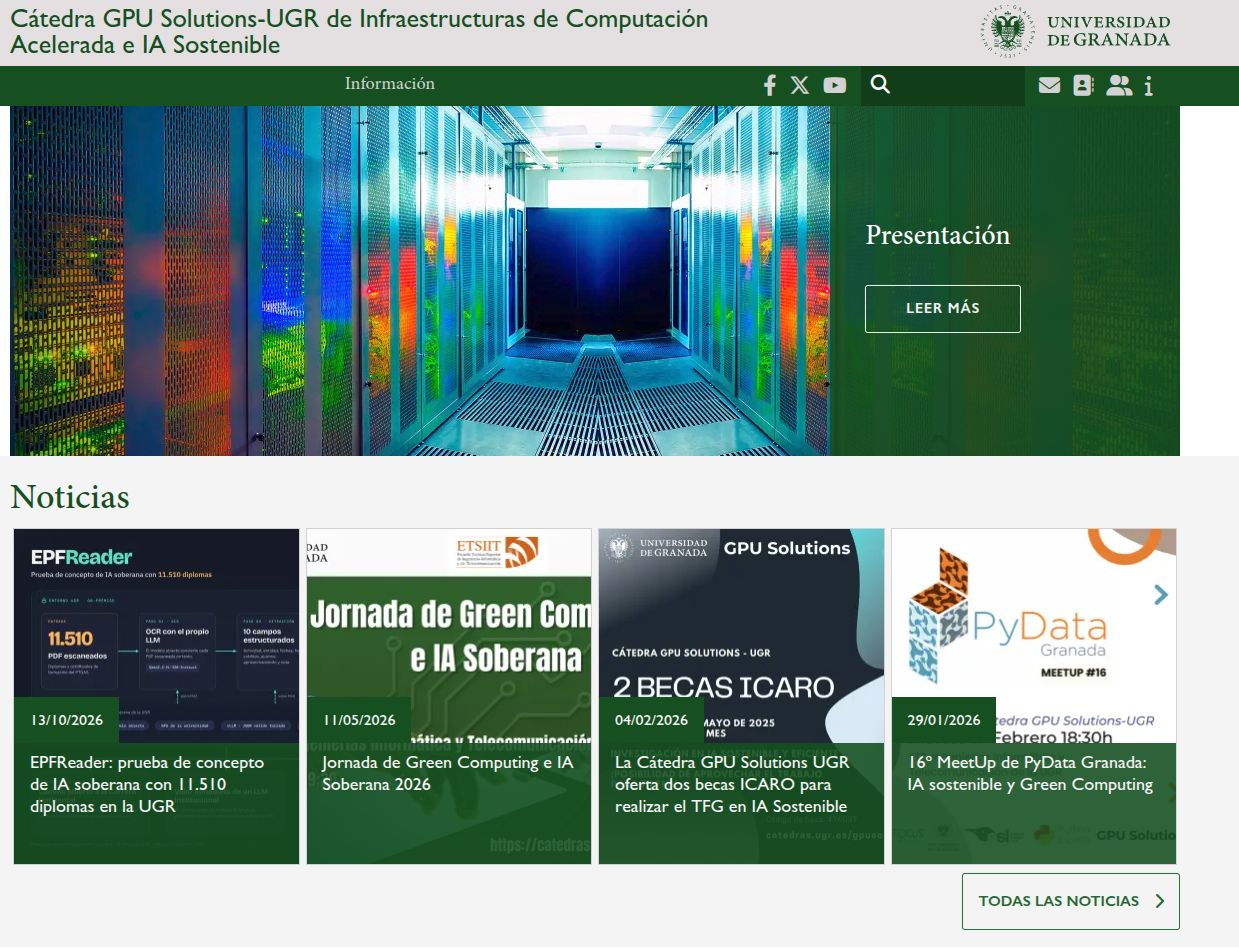
\includegraphics[width=\linewidth,height=5cm,keepaspectratio]{imagenes/catedra.png}\\[6pt]
      {\scriptsize\href{https://catedras.ugr.es/gpusolutions/}{\textcolor{nA}{\texttt{https://catedras.ugr.es/gpusolutions/}}}}
    \end{column}
    \begin{column}{0.45\textwidth}
      \themeblock{rojoUGR}{Gracias}{%
        A la\\\textbf{\mbox{Cátedra GPU Solutions-UGR}}\\
        por el apoyo y el equipamiento facilitado para el desarrollo de MiIA.}
    \end{column}
  \end{columns}
\end{frame}

%=============================================================== cierre
\ugrthanks{¡Gracias!}{¿Preguntas?}{%
  \textbf{Isaac Vidal Daza}\\
  Servicio de Apoyo a la Docencia · CSIRC\\
  \textcolor{rojoUGR}{isvida@ugr.es}\\[12pt]
  {\Large\bfseries\color{ugrInk}   \href{https://www.ugr.es/~isvida}{\texttt{https://www.ugr.es/\raisebox{0.5ex}{\texttildelow}isvida}}}}{}


\end{document}
'
%  Los bloques están en p1_why.tex ... p7_wrapup.tex (se incluyen más abajo).
%  Las ilustraciones van en imagenes/ (ver imagenes/PROMPTS.md); si un fichero
%  no existe, el documento compila igual y muestra un marcador con su nombre.
%
%  Nota: si el entorno no tiene babel-spanish, se usa babel [english] con
%  UTF-8 y sin partición de palabras (la elección es automática).
%==============================================================================
\documentclass[aspectratio=169,11pt]{beamer}
\ifdefined\showpresenternotes
  \setbeameroption{show notes on second screen=right}
\else
  \setbeameroption{hide notes}
\fi

\usepackage[utf8]{inputenc}
\usepackage[T1]{fontenc}
\usepackage{lmodern}
\IfFileExists{spanish.ldf}{%
  \usepackage[spanish,es-noshorthands]{babel}}{%
  \usepackage[english]{babel}\hyphenpenalty=10000 \exhyphenpenalty=10000}
\usepackage{latexUGR}
\usepackage{amssymb}
\usepackage{listings}
\usepackage{array}

\ugrfooter{LLM on-premise · Universidad de Granada}
\ugrlogo{imagenes/logoUGR.png}
\IfFileExists{imagenes/portada.png}{\ugrcover{imagenes/portada.png}}{%
  \IfFileExists{imagenes/portada.jpg}{\ugrcover{imagenes/portada.jpg}}{}}

\title[LLM on-premise]{Infraestructura LLM on-premise}
\subtitle{Inferencia, gateways, agentes y MCP}
\author[I. Vidal Daza]{Isaac Vidal Daza}
\institute[UGR]{Servicio de Apoyo a la Docencia, CSIRC \\ Universidad de Granada}
\date{Máster en Desarrollo del Software · Granada, 2026}

%------------------------------------------------------------------ estilos compartidos
\newcolumntype{R}[1]{>{\raggedright\arraybackslash}p{#1}}

% Diagramas TikZ: cajas planas con borde fino, en la paleta de la plantilla v2
\tikzset{
  bx/.style={rounded corners=4pt, draw=ugrLine, fill=ugrSand, line width=0.8pt,
             align=center, font=\footnotesize, text=ugrInk, inner sep=4pt, minimum height=0.8cm},
  rbx/.style={bx, draw=rojoUGR, fill=rojoUGR!8},
  bbx/.style={bx, draw=nA, fill=nA!8},
  gbx/.style={bx, draw=nB, fill=nB!8},
  pbx/.style={bx, draw=nD, fill=nD!8},
  abx/.style={bx, draw=nE, fill=nE!8},
  ar/.style={-{Stealth[length=4pt]}, line width=0.9pt, draw=ugrText},
  bar/.style={{Stealth[length=4pt]}-{Stealth[length=4pt]}, line width=0.9pt, draw=ugrText},
  lab/.style={font=\footnotesize\itshape, text=darkgray},
}

% Código: fondo arena y barra roja a la izquierda (como la barra del título)
\lstdefinestyle{ugr}{
  basicstyle=\ttfamily\fontsize{6.9}{8.2}\selectfont\color{ugrInk},
  keywordstyle=\color{rojoDark},
  commentstyle=\color{nGreen}\itshape,
  stringstyle=\color{nA},
  backgroundcolor=\color{ugrSand},
  frame=l, framerule=2.5pt, rulecolor=\color{rojoUGR}, framesep=6pt,
  showstringspaces=false, columns=fullflexible, keepspaces=true,
  xleftmargin=10pt, xrightmargin=0pt, aboveskip=2pt, belowskip=2pt,
  breaklines=true, language=Python,
  extendedchars=true, inputencoding=utf8,
  literate={á}{{\'a}}1 {é}{{\'e}}1 {í}{{\'i}}1 {ó}{{\'o}}1 {ú}{{\'u}}1
           {ñ}{{\~n}}1 {Á}{{\'A}}1 {É}{{\'E}}1 {Í}{{\'I}}1 {Ó}{{\'O}}1 {Ú}{{\'U}}1
           {Ñ}{{\~N}}1 {¿}{{?`}}1 {¡}{{!`}}1 {«}{{\guillemotleft}}1 {»}{{\guillemotright}}1
           {·}{{\textperiodcentered}}1 {…}{{\ldots}}1 {→}{{$\rightarrow$}}1
           {ª}{{\textordfeminine}}1,
}
\lstset{style=ugr}

% Chip verde de demo:  \demochip{nombre del script}
\newcommand{\demochip}[1]{%
  \begin{tikzpicture}
    \node[rounded corners=7pt, fill=nB, text=white, font=\scriptsize\bfseries,
          inner xsep=7pt, inner ysep=3pt]
      {$\blacktriangleright$\ Demo: \texttt{#1}};
  \end{tikzpicture}}
\newcommand{\demoline}[1]{\par\vspace{2pt}\hfill\demochip{#1}\par}

% Línea de fuentes al pie de un frame
\newcommand{\srcline}[1]{{\par\vspace{2pt}\tiny\color{darkgray}Fuentes: #1\par}}

% Ilustración con marcador: usa imagenes/<fichero> si existe; si no, muestra un
% recuadro con el nombre y la descripción (así el documento siempre compila).
%   \imgslot{fichero}{ancho}{alto}{descripción del marcador}
\newcommand{\imgslot}[4]{%
  \IfFileExists{imagenes/#1}{%
    \includegraphics[width=#2,height=#3,keepaspectratio]{imagenes/#1}}{%
    \begin{tikzpicture}
      \node[draw=darkgray!50, dashed, line width=0.8pt, fill=ugrSand, rounded corners=5pt,
            minimum width=#2, minimum height=#3, text width=\dimexpr#2-0.8cm\relax,
            align=center, text=darkgray, font=\scriptsize]
        {\textbf{Imagen pendiente}\\[1pt] \texttt{\detokenize{imagenes/#1}}\\[3pt] #4};
    \end{tikzpicture}}}

\begin{document}

%--------------------------------------------------------------- portada
\newcommand{\portadarepo}{%
  \tikz[remember picture,overlay] \node[anchor=south west,inner sep=0pt,align=left]
    at ([xshift=4.2cm,yshift=0.7cm]current page.south west)
    {\footnotesize Presentación, código y ejemplos:\\
     \footnotesize\color{nA}\href{https://github.com/isvida/MiIA-demo}{\texttt{https://github.com/isvida/MiIA-demo}}};}
\ugrtitleframe[\ugrtag{Inferencia}\hspace{4pt}\ugrtag{Pasarela}\hspace{4pt}\ugrtag{Agentes}\hspace{4pt}\ugrtag{MCP}\smash{\portadarepo}]

%--------------------------------------------------------------- frase de apertura
\ugrstatement{Un modelo de lenguaje ya no es un experimento: es una pieza más de la infraestructura, como el correo o las bases de datos.}{Punto de partida de este seminario}

%--------------------------------------------------------------- agenda
\begin{frame}{Agenda}{Tiempo transcurrido previsto al comenzar cada bloque · formato h:mm}
	\note{Dos horas; señalar el orden y las demos.}
	\vspace{0.1cm}
	\begin{tikzpicture}
		\foreach \n/\t/\m/\p [count=\i] in {
		1/{¿Por qué tener tu propio LLM?}/{0:00}/{},
		2/{Motores de inferencia}/{0:10}/{01\_hola\_api · 02\_concurrencia},
		3/{Hablar con un LLM}/{0:30}/{03\_salida · 04\_tool\_calling},
		4/{Arquitectura del servicio}/{0:45}/{pasarela, claves, respaldo},
		5/{Agentes, MCP y skills}/{1:05}/{05\_agente · 06\_agente\_mcp},
		6/{Casos de uso}/{1:30}/{03 (patrón EPFReader)},
		7/{Conclusiones y preguntas}/{1:50}/{}}{
		\pgfmathsetmacro{\yy}{-(\i-1)*0.62}
		\node[fill=rojoUGR, text=white, font=\scriptsize\bfseries, minimum size=0.48cm,
			rounded corners=1.5pt, anchor=west] at (0,\yy) {\n};
		\node[anchor=west, text=ugrInk, font=\normalsize\bfseries] at (0.75,\yy) {\t};
		\node[anchor=east, text=rojoUGR, font=\small\bfseries] at (8.3,\yy) {\m};
		\node[anchor=west, text=darkgray, font=\scriptsize] at (8.8,\yy) {\p};
		}
		\draw[ugrLine, line width=1pt] (0,-4.15) -- (13.8,-4.15);
		\node[anchor=west, text=ugrInk, font=\normalsize\bfseries] at (0.75,-4.5) {Fin previsto};
		\node[anchor=east, text=rojoUGR, font=\small\bfseries] at (8.3,-4.5) {2:00};
	\end{tikzpicture}
\end{frame}

%--------------------------------------------------------------- puesta en marcha
\begin{frame}[fragile]{Antes de empezar: levanta la demo}{Una miniatura de la infraestructura real, sin necesidad de GPU}
	\note{Dejar la descarga en marcha; servicios locales y URL de acceso.}
	\begin{columns}[T]
		\begin{column}{0.56\textwidth}
			\begin{lstlisting}[language={}]
unzip miia-demo.zip && cd miia-demo
docker compose pull
docker compose build
docker compose up -d
docker compose run --rm lab \
    python ejemplos/01_hola_api.py
\end{lstlisting}
			\vspace{6pt}
			{\footnotesize Requiere Docker con Compose v2, unos 8 GB de RAM libres y unos 6 GB de disco.
				Hay un perfil opcional con GPU y vLLM.}
		\end{column}
		\begin{column}{0.42\textwidth}
			\themeblock{nA}{Qué se levanta, y dónde}{%
				Chat (Open WebUI): \texttt{localhost:3000}\\
				Panel de LiteLLM: \texttt{localhost:4000/ui}\\
				API tipo OpenAI: \texttt{localhost:4000/v1}\\
				Servidor MCP: \texttt{localhost:8001/mcp}}
		\end{column}
	\end{columns}
	\keymsg{Lanza la descarga ya: se completa mientras vemos el bloque 1.}
\end{frame}

%--------------------------------------------------------------- bloques
\InputIfFileExists{p1_why.tex}{}{}
\InputIfFileExists{p2_inference.tex}{}{}
\InputIfFileExists{p3_api.tex}{}{}
\InputIfFileExists{p4_architecture.tex}{}{}
\InputIfFileExists{p5_agents.tex}{}{}
\InputIfFileExists{p6_usecases.tex}{}{}
\InputIfFileExists{p7_wrapup.tex}{}{}

%--------------------------------------------------------------- invitación al MOOC
\ugrimageframe{imagenes/equipo_gobierno_mia.png}
  {¿Podría MiIA tomar el control de la UGR y sustituir al equipo de gobierno?}
  {Una pregunta para mirar más allá de la automatización.}

\ugrimageframe{imagenes/mooc.png}
  {¿Quieres la respuesta? Apúntate al MOOC del CEPRUD}
  {\footnotesize Capítulo: Inteligencia artificial y evolución: modelando un sistema vivo artificial\\
   Coorganizan: Isaac Vidal Daza y Mónica Sánchez-Román (Mineralogía y Petrología, UGR)\\
   Posible apertura de matrícula en diciembre.}

\begin{frame}{Agradecimientos}{CSIRC · Apoyo a la Docencia}
  \note{Equipo de apoyo a la docencia del CSIRC.}
  \centering
  \begin{tikzpicture}[
    persona/.style={bx, text width=3.4cm, minimum height=0.7cm,
                    font=\footnotesize, inner sep=3pt},
    centro/.style={rbx, text width=3.0cm, minimum height=1.0cm,
                   font=\small\bfseries, inner sep=4pt},
    enlace/.style={draw=ugrLine, line width=0.9pt}
  ]
    \node[centro] (francisco) at (0,0) {Francisco Manuel\\Romera Juárez};
    \node[persona] (domingo) at (-4.2,1.5) {Domingo de Guzmán\\Baca Ruiz};
    \node[persona] (antonio) at (-4.2,0.5) {Antonio Ángel\\Cano Ruano};
    \node[persona] (rodrigo) at (-4.2,-0.5) {Rodrigo González\\Gálvez};
    \node[persona] (fernando) at (-4.2,-1.5) {Fernando Antonio\\López Álvarez};
    \node[persona] (leire) at (4.2,1.5) {Leire Melchor López};
    \node[persona] (gines) at (4.2,0.5) {Ginés Rubio Flores};
    \node[persona] (ruiz) at (4.2,-0.5) {Antonio Ruiz González};
    \node[persona] (isaac) at (4.2,-1.5) {Isaac Vidal Daza};
    \begin{scope}[on background layer]
      \foreach \persona in {domingo,antonio,rodrigo,fernando,leire,gines,ruiz,isaac}
        \draw[enlace] (francisco) -- (\persona);
    \end{scope}
  \end{tikzpicture}

  \vspace{3pt}
  {\scriptsize Centro de Servicios Informáticos y Redes de Comunicación\\
  Servicio Central de Informática (Edf. Mecenas) · C/ Profesor Adolfo Rancaño,
  18071 Granada\\
  \href{http://csirc.ugr.es}{\textcolor{nA}{csirc.ugr.es}}}
\end{frame}

\begin{frame}{Agradecimientos}{Cátedra GPU Solutions-UGR}
  \note{Agradecer el apoyo y el equipamiento de la Cátedra.}
  \begin{columns}[c]
    \begin{column}{0.53\textwidth}
      \centering
      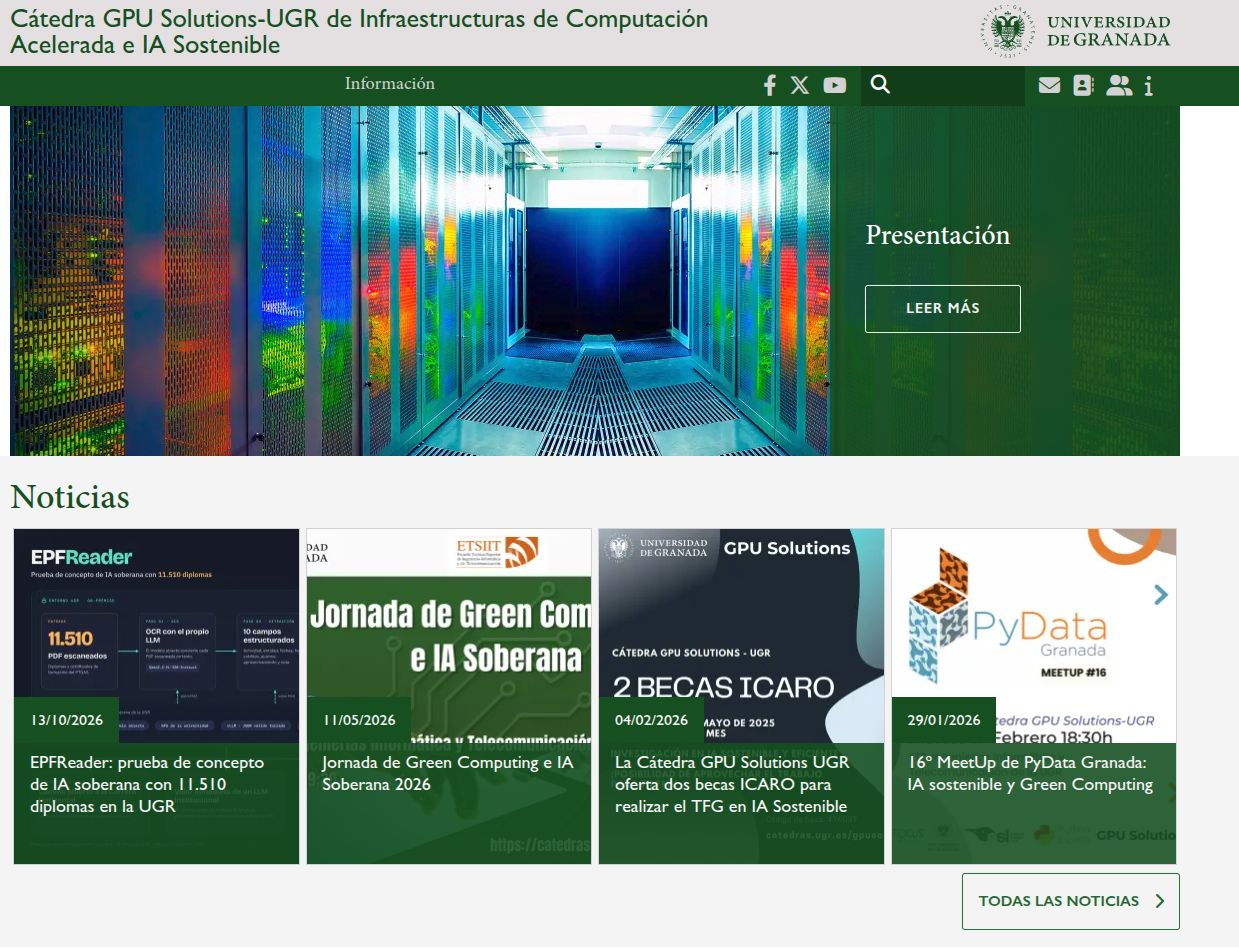
\includegraphics[width=\linewidth,height=5cm,keepaspectratio]{imagenes/catedra.png}\\[6pt]
      {\scriptsize\href{https://catedras.ugr.es/gpusolutions/}{\textcolor{nA}{\texttt{https://catedras.ugr.es/gpusolutions/}}}}
    \end{column}
    \begin{column}{0.45\textwidth}
      \themeblock{rojoUGR}{Gracias}{%
        A la\\\textbf{\mbox{Cátedra GPU Solutions-UGR}}\\
        por el apoyo y el equipamiento facilitado para el desarrollo de MiIA.}
    \end{column}
  \end{columns}
\end{frame}

%=============================================================== cierre
\ugrthanks{¡Gracias!}{¿Preguntas?}{%
  \textbf{Isaac Vidal Daza}\\
  Servicio de Apoyo a la Docencia · CSIRC\\
  \textcolor{rojoUGR}{isvida@ugr.es}\\[12pt]
  {\Large\bfseries\color{ugrInk}   \href{https://www.ugr.es/~isvida}{\texttt{https://www.ugr.es/\raisebox{0.5ex}{\texttildelow}isvida}}}}{}


\end{document}
